\phantom.
\vspace{3cm}
\section{Results}\label{sec_phass}
In this chapter, the results obtained within this thesis are presented, which can be be divided into three parts: In the first part, a general first-principles formalism is developed allowing for the inclusion of electron-phonon interactions (EPI) into the solution of the Bethe-Salpeter equation (BSE).  In the second part, the developed formalism is applied to the case of polar crystals where strong Fr\"ohlich coupling is present. The numerical evaluation of the developed formalism constitutes the third part. Here, the impact of EPI on excitonic binding energies is studied for various polar insulators and semiconductors.

%---------------------------------
\subsection{Phonon contribution to the screened Coulomb interaction}\label{ph_contrib_sec}
%---------------------------------

 %-----------------
\subsubsection{Real-space formulation}
%-----------------

From Section~\ref{epi_el}, we recall that the phonon contribution to the screened Coulomb interaction (Eq.\;\ref{wph_time_domain}) is given by 
%

\begin{equation}\nonumber
      W^\text{ph}(1,2) =  \sum_{\nu\nu'}\int\!\!\int_{\Omega_\text{BZ}}\frac{\text{d}\omega}{2\pi}\frac{\text{d}\q}{\Omega_\text{BZ}}\,e^{-i\omega(t_2-t_1)}\,
 g^\text{cc}_{\q\nu}(\r_2,\omega)\, D_{\q\nu\nu'}(\omega)\,g_{\q\nu'}(\r_1,\omega),
\end{equation}
%
with the  fully interacting phonon propagator $D_{\q\nu\nu'}(\omega)$ and the screened electron-phonon coupling functions $g_{\q\nu}(\r,\omega)$ and $g^\text{cc}_{\q\nu}(\r,\omega)$ (Eqs.\;\eqref{eph_coupl_func} and \eqref{eph_coupl_func_cc}). The reciprocal integration extends over the first Brioullin 
zone with volume~$\Omega_\text{BZ}$.\par
In order to make Eq.\;\ref{wph_time_domain} amenable to first-principles calculations, it is common \cite{Giustino} to make the following two approximations: First, the frequency dependence of the coupling function is neglected and only the static limit is considered. Since the dielectric matrix is real at $\omega=0$, we have the simple relation
\begin{equation}
    g^\text{cc}_{\q\nu}(\r,0) = g^*_{\q\nu}(\r,0).
\end{equation}
%
Second, the fully interacting phonon propagator $D_{\q\nu\nu'}(\omega)$ is replaced by its adiabatic counterpart $D^\text{A}_{\q\nu}(\omega)$, which is diagonal in the phonon modes ($\eta \rightarrow 0^+$):
%
\begin{align}\label{adiab_prop}
    D^\text{A}_{\q\nu}(\omega) = \frac{1}{\omega - \omega_{\q\nu} + i\eta} - \frac{1}{\omega + \omega_{\q\nu} - i\eta}.
\end{align}
%
In view of practical calculations, we replace the integration in reciprocal space by a summation over discrete points, \textit{i.e.}, ${\int\frac{d\q}{\Omega_\text{BZ}}\rightarrow N^{-1}_p\sum_{\q\in\text{BZ}}}$, where $N_p$ is the number of points in the $\q$-grid. The screened Coulomb interaction then reads
%
\begin{subequations}\label{w_realspace_set}
\begin{align}
 W^\text{ph}(\r_1,\r_2,\omega) & = N^{-1}_p\,\sum^\text{BZ}_{\q}\sum_\nu W_{\q\nu}(\r_1,\r_2)\,D^\text{A}_{\q\nu}(\omega)\label{w_realspace}\\[10pt]
 W_{\q\nu}(\r_1,\r_2) & = g^*_{\q\nu}(\r_2)\,g_{\q\nu}(\r_1)\label{w_spat_behvaiour},
\end{align}
\end{subequations}
%
where we introduced $W_{\q\nu}(\r_1,\r_2)$ as the spatial contribution of a phonon mode ${\q\nu}$ to $W^\text{ph}(\r_1,\r_2,\omega) $. This will be helpful, on the one hand, to keep the notation more compact and, on the other hand, to stress similarities with the electronic part of $W$ in the following derivations.  Due to the symmetry of the lattice, the coupling function $g$ can be written as a Bloch wave:
%
\begin{equation}\label{blochcoupl}
     g_{\q\nu}(\r) = e^{i\mathbf{q\cdot r}}\Delta_\text{P}^{\!\q\nu}v      ^{\phantom{I}}_\text{KS}(\r),
\end{equation}
%
where $\Delta_\text{P}^{\!\q\nu}v^{\phantom{I}}_\text{KS}(\r)$ is the lattice-periodic part of the coupling function\cite{Giustino}. It can now be verified that  $W^\text{ph}$ is periodic with respect to a shift of both arguments by the same lattice vector $\R$, \textit{i.e.},
%
\begin{equation}\label{w_periodic}
     W^\text{ph}(\r_1,\r_2,\omega) = W^\text{ph}(\r_1 + \R,\r_2 + \R,\omega).
\end{equation}
%
It should be stressed that the definition of $W^\text{ph}$ in Eq.\;\eqref{w_realspace} includes the coupling to all phonon modes of the crystal. This is a significant difference from simplifying screening models as the one presented in Section~\ref{subsec_scrcoulint} where the coupling to only one specific phonon mode is assumed.

%-------------------------------------
\subsubsection{Fourier representation}
%-------------------------------------

 Since the contribution of phonons to the screened Coulomb interaction is lattice periodic as shown in Eq.\;\eqref{w_periodic}, its Fourier coefficients can be computed according to  the convention \eqref{fourier_coeff} as 
%
\begin{equation}\label{w_fourier_coeff}
      W^\text{ph}_\mathbf{GG'}(\q,\omega) = \frac{1}{V}\int\!\!\int_V \text{\!\!d}\r_1\text{d}\r_2\,e^{-i\mathbf{(q+G)\cdot r}_1}\,W^\text{ph}(\r_1,\r_2,\omega)\,e^{i\mathbf{(q+G')\cdot r}_2}.
\end{equation}
%
The two spatial integrations are independent due to the definition of $W^\text{ph}$ in Eqs.~\eqref{w_realspace} and \eqref{w_spat_behvaiour}. Therefore, it is convenient to introduce the Fourier coefficient of the coupling function~as 
%
\begin{align}\label{coupling_fourier}
     \Tilde{g}_{\mathbf{q'}\nu}^{\G}(\q) = \frac{1}{V} \int_V \text{\!\!d}^3\r\, g_{\mathbf{q'}\nu}(\r)\,e^{-i(\q+\G)\cdot\r}\,\delta_\mathbf{qq'}.
\end{align}
%
 One may verify that only terms for which $\mathbf{q=q'}$ are nonvanishing by exploiting the property of the coupling function as a Bloch wave as shown in  Eq.\;\eqref{blochdelta}.
Equation\;\eqref{w_fourier_coeff} can now be rewritten by inserting the  expression of $W^\text{ph}$ in real space (Eq.\;\eqref{w_realspace}) and making use of the Fourier transform defined in Eq.\;\eqref{coupling_fourier}:
%
\begin{align}\label{w_fourier_coeff3}
   W^\text{ph}_{\G\G'}(\q,\omega) = \frac{V}{N_p}\sum_{\nu} \Tilde{g}_{\q\nu}^{\G}(\q)\left[\Tilde{g}_{\q\nu}^{\G'}(\q)\right]^*D^A_{\q\nu}(\omega). 
\end{align}
%
The prefactor $V/N_p=\Omega_\text{UC}$ simply gives the unit cell volume.

\subsubsection{Expansion of the coupling function}
To make a connection between the theory developed within this thesis and the standard formulation of EPI in terms of electron-phonon matrix elements (defined in Section~\ref{subsec_epc}), we expand the coupling function in real space in terms of single-particle electronic wave functions.\par 
To carry out the expansion, a local operator $\hat{g}_{\q\nu}$ is defined. Its matrix elements in real space are denoted as $g^{(2)}_{\q\nu}(\mathbf{r,r'})$ and are related to the coupling function by
%
\begin{align}
    \mel{\r}{\hat{g}_{\q\nu}}{\mathbf{r'}} = g^{(2)}_{\q\nu}(\mathbf{r,r'}) = g_{\q\nu}(\r)\,\delta(\mathbf{r-r'}).
\end{align}
%
An expansion into single-particle wave functions is possible by inserting twice the completeness relation $ \hat{\mathbb{1}} = \sum_{n\k}\ket{\psi_{n\k}}\bra{\psi_{n\k}}$.
%
The preceding expression can then be expanded as 
%
\begin{align}\label{double_exp}
    g^{(2)}_{\q\nu}(\mathbf{r,r'}) = \sum_{n\k}\sum_{m\mathbf{k'}} \mel{\psi_{m\mathbf{k'}}}{\hat{g}_{\q\nu}}{\psi_{n\k}}\psi_{m\mathbf{k'}}(\r)\,\psi^*_{n\k}(\mathbf{r'}),
\end{align}
%
where the matrix element on the right-hand side can be identified as the electron-phonon coupling element $g_{\nu mn}(\mathbf{k,k',q})$ defined in Eq.\;\eqref{g_coupl_func} for $\mathbf{k'=k+q}$. As it will become clear later, it is helpful to keep the crystal momenta independent, such that formally the matrix element depends on two independent electron momenta.\par 
To obtain the Fourier coefficients of the coupling function using the expansion in Eq.\;\eqref{double_exp}, we rewrite the Fourier transformation in Eq.\;\eqref{coupling_fourier} as
%
\begin{align}\label{double_fourier}
     \Tilde{g}_{\q\nu}^{\G}(\q) = \frac{1}{V} \int\!\!\int_V\text{\!\!d}^3\r \text{d}^3\mathbf{r'} \,g^{(2)}_{\q\nu}(\mathbf{r,r'})\,e^{-i(\q+\G)\cdot\r}.
\end{align}
%
Moreover, for the sake of a compact notation, we define the Fourier transform $\Tilde{\psi}$ of a wave function as
%
\begin{align}\label{fourier_wave}
    \Tilde{\psi}_{n\k}^\G(\q) = \frac{1}{V}\int_V\text{\!\!d}^3\r\,e^{-i(\q+\G)\cdot\r}\,\psi_{n\k}(\r).
\end{align}
%
After inserting the expansion in Eq.\;\eqref{double_exp} inside Eq.\;\eqref{double_fourier} and making use of the definition in Eq.\;\eqref{fourier_wave}, we can rewrite Eq.\;\eqref{w_fourier_coeff3} as
%
\begin{subequations}\label{w_fourier_set}
\begin{align}
   W^\text{ph}_{\G\G'}(\q,\omega) & = \Omega_\text{UC} \sum_\nu   W_{\q\nu}^{\G\G'}\!(\q)\,D^A_{\q\nu}(\omega) \label{w_fourier_final}\\[10pt]
    W_{\q\nu}^{\G\G'}\!(\q) & =\Tilde{g}_{\q\nu}^{\G}(\q)\left[\Tilde{g}_{\q\nu}^{\G'}(\q)\right]^* \label{w_fourier_spatial} \\[16pt]
   \Tilde{g}_{\q\nu}^{\G}(\q) & = V\sum_{n\k}\sum_{m\mathbf{k'}}g_{\nu mn}(\mathbf{k,k',q}) \,\Tilde{\psi}_{m\k'}^{\G}(\q) \left[\Tilde{\psi}_{n\k}^{0}(0)\right]^*\label{g_fourier_final}.
   \end{align}
\end{subequations}
%
In order to keep the notation as it used in  Eq.\;\eqref{w_realspace}, $ W_{\q\nu}^{\G\G'}\!(\q)$ is introduced as the Fourier coefficient of the spatial contribution $W_{\q\nu}(\r_1,\r_2)$ of a single phonon mode~$\q\nu$. 

%-------------------------------------
\subsubsection{Contribution to the direct BSE term}\label{dir_int_ph}
%-------------------------------------

Thus far, we have derived an expression for the Fourier coefficients of the lattice-induced part of the screened Coulomb interaction. To do calculations within the BSE formalism, we need to evaluate their influence on the total direct interaction term. Similar to the total $W$ in Eq.\;\eqref{total_w}, the total direct term is the sum of an electronic  contribution $H^\text{el}$ and  a contribution $H^\text{ph}$ stemming from the coupling to phonons:
%
\begin{equation}\label{hdir_tot}
    H^\text{dir}_{vc\k,v'c'\k'} = H^\text{el}_{vc\k,v'c'\k'} + H^\text{ph}_{vc\k,v'c'\k'}.
\end{equation}
%
\newpage
The direct interaction term including dynamical screening is given in Eq.\;\eqref{screen_dyn}. Using the expressions for the Fourier coefficients of $W^\text{ph}$ according to Eq.\;\eqref{w_fourier_final}, one finds that the lattice vibrations give the following contribution:
%
\begin{equation}
\begin{aligned}\label{h_nu_fourier}
    H^\text{ph}_{vc\k,v'c'\k'}  = &  \frac{1}{V}\sum_\nu\sum_{\mathbf{GG'}}  W_{\q\nu}^{\G\G'}\!(\q)\,M^\G_{cc'}(\mathbf{k,q})\,[M^\mathbf{G'}_{vv'}(\mathbf{k,q})]^*\\[10pt]
     & \times \frac{i}{2\pi}\int\text{\!\!d}\omega\,e^{-i\omega\eta}  \Biggl[\frac{1}{\omega - \omega_{\q\nu} + i\eta} - \frac{1}{\omega + \omega_{\q\nu} - i\eta}\Biggr] \\[10pt]
     & \times \Biggl[\frac{1}{  E^\lambda - \left(\varepsilon^\text{QP}_{c\k} - \varepsilon^\text{QP}_{v'\mathbf{k'}}\right)  - \omega + i\eta } \\[10pt]
     & + \frac{1}{ E^\lambda - \left(\varepsilon^\text{QP}_{c'\mathbf{k'}} - \varepsilon^\text{QP}_{v\k}\right) + \omega +  i\eta}\Biggr],
\end{aligned}
\end{equation}
 %
where here and in the following equations the different wave vectors are related by $\mathbf{k'=k+q}$.
The definition of the adiabatic phonon propagator (Eq.\;\eqref{adiab_prop}) was~inserted.\par
\noindent We now move to the complex plane ($\omega\rightarrow z$) to evaluate the frequency integral in Eq.\;\eqref{h_nu_fourier} as a contour integral, which allows the use of the residue theorem (see Appendix\;\ref{residue}). We have to solve the following contour integral:
%
\begin{equation}
         I =  \frac{i}{2\pi}\int_C\text{d}z\,f(z),
\end{equation}
where 
\begin{equation}
  \begin{aligned}
      f(z) = e^{-iz\eta} & \left[\frac{1}{z - \omega_{\q\nu} + i\eta} - \frac{1}{z + \omega_{\q\nu} - i\eta}\right]\\[10pt]
       \times & \Biggl[\frac{1}{ E^\lambda - \left(\varepsilon^\text{QP}_{c\k} - \varepsilon^\text{QP}_{v'\mathbf{k'}}\right) - z
       + i\eta} + \frac{1}{  E^\lambda - \left(\varepsilon^\text{QP}_{c'\mathbf{k'}} - \varepsilon^\text{QP}_{v\k}\right) + z + i\eta}\Biggr].\\[10pt]
 \end{aligned}
 \end{equation}
%
Due to the complex exponential, the contour can be closed in the lower half of the complex plane where the integral vanishes. The contour and the poles of $f$ in the complex plane are sketched in Figure~\ref{contour}. The integrand has four poles lying in the complex plane, which are given by
%
\begin{align}
    z_1 & = E^\lambda - \left(\varepsilon^\text{QP}_{c\k} - \varepsilon^\text{QP}_{v'\mathbf{k'}}\right) + i\eta,  && z_2 = -\omega_{\q\nu} + i\eta \\[10pt]
      z_3 & =\omega_{\q\nu} - i\eta,  && z_4 =  - E^\lambda + \left(\varepsilon^\text{QP}_{c'\mathbf{k'}} - \varepsilon^\text{QP}_{v\k}\right) - i\eta.
\end{align}
%
 \begin{figure}[t]
\centering
\begin{tikzpicture}[node distance=8cm]
\node (xstart) {};
\node (xend) [right of=xstart] {Re $z$};
\node (ystart) [below of=xstart, xshift = 4 cm, yshift =  + 5cm] {};
\node (yend) [above of=ystart,yshift=-2cm] {Im $z$};
\node (center)[above of=ystart,xshift=3cm,yshift=-5cm] {};
\node (pole1) [above of =xstart, xshift = 3cm,yshift = -7.5cm,  circle,fill,inner sep=1.5pt]{};
\node (text1) [above of =xstart, xshift = 3cm,yshift = -7cm]{$z_2$};

\node (pole2) [above of =xstart, xshift = 2cm,yshift = -7.5cm,  circle,fill,inner sep=1.5pt]{};
\node (text1) [above of =xstart, xshift = 2cm,yshift = -7cm]{$z_1$};

\node (pole3) [above of =xstart, xshift = 5cm,yshift = -8.5cm,  circle,fill,inner sep=1.5pt]{};
\node (text3) [above of =xstart, xshift = 5cm,yshift = -9cm]{$z_3$};
\node (pole4) [above of =xstart, xshift = 6cm,yshift = -8.5cm,  circle,fill,inner sep=1.5pt]{};
\node (text4) [above of =xstart, xshift = 6cm,yshift = -9cm]{$z_4$};
\node (linepoint) [above of =xstart, xshift = 5.5cm,yshift = -8cm]{};

\node (text4) [above of =xstart, xshift = 6.5cm,yshift = -10cm]{$C$};

\draw  [->,>=stealth',very thick]   (xstart) -- (linepoint.center) ;
\draw [line]   (linepoint.center) -- (xend) ;
\draw [line]   (ystart) -- (yend) ;
\draw [->,>=stealth',very thick] (center) arc (-10:-170:3cm);
\end{tikzpicture}

\caption{\label{contour} Analytical structure of $f(z)$ in the complex plane.}
\end{figure}
%

Since the contour is closed in the lower half of the complex plane, only the residues of the third and the fourth pole will contribute to the integral through
%
\begin{align}\label{intomega}
     I = \frac{i}{2\pi} \left[ 2\pi\,i\, \underset{z=z_3}{\text{Res}}\,f(z) + 2\pi\,i\,\ \underset{z=z_4}{\text{Res}}\,f(z)\right].
\end{align}
 %
According to Eq.\;\eqref{residue_pole}, the residues of a simple pole $z_i$ can be obtained by 
%
\begin{equation}
    \underset{z=z_i}{\text{Res}}\,f(z) = \lim_{z\rightarrow z_k}(z-z_i)\,f(z).
\end{equation}
 %
 In the present case, one obtains for the residues at poles $z_3$ and $z_4$ 
 %
 \begin{align}
    \underset{z=z_3}{\text{Res}}\,f(z) & =\left[ E^\lambda - \left(\varepsilon^\text{QP}_{c\k} - \varepsilon^\text{QP}_{v'\mathbf{k'}}\right) - \omega_{\q\nu}\right]^{-1} + \left[  E^\lambda - \left(\varepsilon^\text{QP}_{c'\mathbf{k'}} - \varepsilon^\text{QP}_{v\k}\right) + \omega_{\q\nu}\right]^{-1} \\[10pt]
     \underset{z=z_4}{\text{Res}}\,f(z) &  =  \left[ E^\lambda - \left(\varepsilon^\text{QP}_{c'\mathbf{k'}} - \varepsilon^\text{QP}_{v\k}\right) - \omega_{\q\nu} \right]^{-1} - \left[ E^\lambda - \left(\varepsilon^\text{QP}_{c'\mathbf{k'}} - \varepsilon^\text{QP}_{v\k}\right) + \omega_{\q\nu}\right]^{-1}.
 \end{align}
 %
 Adding up the residues according to Eq.\;\eqref{intomega}, the result of the integral is
 %
 \begin{equation}
     I = \left[\omega_{\q\nu}  + \left(\varepsilon^\text{QP}_{c\k} - \varepsilon^\text{QP}_{v'\mathbf{k'}}\right) - E^\lambda  \right] ^{-1} + \left[ \omega_{\q\nu} + \left(\varepsilon^\text{QP}_{c'\mathbf{k'}} - \varepsilon^\text{QP}_{v\k}\right) - E^\lambda \right]^{-1}.
 \end{equation}
 %
 \newpage Finally, we can plug in this result inside Eq.\;\eqref{h_nu_fourier} to obtain the following expression for the phonon contribution of the direct term:
%
\begin{equation}\label{h_dir_final}
\begin{aligned}
   H^\text{ph}_{vc\k,v'c'\k'}  = &  \frac{1}{V}\sum_\nu\sum_{\mathbf{GG'}}\frac{2}{\omega_{\q\nu}} W_{\q\nu}^{\G\G'}\!(\q)\,M^\G_{cc'}(\mathbf{k,q})\,[M^\mathbf{G'}_{vv'}(\mathbf{k,q})]^*\\[10pt]
     & \times \frac{\omega_{\q\nu}}{2}\Bigg[\frac{1}{\omega_{\q\nu}  + \left(\varepsilon^\text{QP}_{c\k} - \varepsilon^\text{QP}_{v'\mathbf{k'}}\right) - E^\lambda  } \\[10pt]
      & +  \frac{1}{  \omega_{\q\nu} + \left(\varepsilon^\text{QP}_{c'\mathbf{k'}} - \varepsilon^\text{QP}_{v\k}\right) -  E^\lambda }\Bigg].
\end{aligned}
\end{equation}
%
In order to illustrate the dynamics more clearly, the expression was extended by $2/\omega_{\q\nu}$ in the first line and the corresponding inverse in the third line. The second and third line in Eq.\;\eqref{h_dir_final} then yield a factor in the interval (0,1) weighting the contribution of each mode. In the limit of large phonon frequencies, \textit{i.e.}, $ \omega_{\q\nu}\gg\varepsilon^\text{QP}_{c'\mathbf{k'}} - \varepsilon^\text{QP}_{v\k} -  E^\lambda$, the mode can fully contribute to the screening and the weighting factor becomes equal to one. In the limit of small phonon frequencies, $ \omega_{\q\nu}\ll\varepsilon^\text{QP}_{c'\mathbf{k'}} - \varepsilon^\text{QP}_{v\k} -  E^\lambda$ holds and the mode is not able to follow the exciton formation at all.  The weighting factor accordingly vanishes in this case. Thus, we find that the lattice fully contributes to the screening if the excitonic binding energy is small compared to the phonon frequencies and that, in the opposite limit, the lattice does not contribute to the screening at all.  In all other cases, each mode contributes partially to the screening.\par 
It should be noted that the derivation so far is completely general and no assumptions about the character of the electron-phonon coupling are made. To do quantitative calculations, the electron-phonon matrix element $g_{\nu mn}$ has to be given, which will depend on the material to be studied. 


%--------------------
%--------------------
\subsection{Application to polar crystals}\label{pol_ph_sec}
%--------------------
%--------------------
In the preceding section, general expressions accounting for the contribution of phonons to the screened Coulomb interaction and to the direct BSE term were developed.  In this section, we will focus on polar insulators and semiconductors, where the coupling of electrons to long-range longitudinal-optical (LO) phonons dominates. To study materials on a computational basis, this interaction needs to be specified in terms of an electron-phonon matrix element. In polar materials, an explicit expression capturing the long-range interaction exists, which is a generalization of the well-known (original) Fr\"ohlich vertex described in Section~\ref{subsec_frohlich}.  Under the assumptions made in the original work\cite{froehlich}, a widely-used screening model can be recovered.

%--------------------
\subsubsection{Generalized Fr\"ohlich coupling}
%--------------------

In polar materials, at least two atoms in the unit cell carry nonvanishing Born effective charges\cite{gonze_lee}. This results in the Fr\"ohlich interaction, which describes the coupling of electrons and holes to macroscopic electric fields generated by LO phonons. The expression derived in the original work\cite{froehlich} described in Section~\ref{subsec_frohlich}, considering an isotropic system with a dispersionless LO phonon, has been generalized\cite{gius_verdi} in order to define the Fr\"ohlich coupling in a way that includes the coupling to all phonon modes and allows the description of anisotropic materials. Within the generalized approach, the total coupling element is given as a sum of a long- ($\mathcal{L}$) and a short-range ($\mathcal{S}$) part:
%
\begin{align}
    g_{\nu mn}(\mathbf{k,q}) = g^{(\mathcal{S})}_{\nu mn}(\mathbf{k,q}) + g^{(\mathcal{L})}_{\nu mn}(\mathbf{k,q}).
\end{align}
The long-range part corresponds to the original Fr\"ohlich coupling and contains all contributions leading to the divergence at small $\q$, such that the short-range part will be finite. This approach is comparable to the calculation of LO-TO splitting in polar materials by separating the analytical and nonanalytical parts of the interatomic force constants (see Section~\ref{pol_phon}). The long-range component of the matrix element reads
%
\begin{equation}\label{frohlich_mel}
  g^{(\mathcal{L})}_{\nu mn}(\mathbf{k,q}) = i B_{\q\nu}\sum_\mathbf{G\neq -q}\mathbf{C(q+G)}\cdot\bar{\mathbf{Q}}_{\nu\G}(\q) \mel{\psi_{m\mathbf{k+q}}}{e^{i\mathbf{(q+G)\cdot r}}}{\psi_{n\k}}.
\end{equation}
%
The appearing quantities are defined by
%
\begin{subequations}\label{subequ_glr}
\begin{align}
B_{\q\nu} & = \frac{4\pi}{\Omega_\text{UC}} \left( \frac{1}{2\omega_{\q\nu}}   \right)^{\!\!1/2}\label{comp1}\\[10pt]
\mathbf{C(q+G)} & = \frac{\mathbf{(q+G)}}{\mathbf{(q+G)}\cdot\boldsymbol{\varepsilon}_\infty\cdot\mathbf{(q+G)}} = \frac{\mathbf{X}_\G(\boldsymbol{\varepsilon}_\infty,\q)}{|\mathbf{q+G}|} \label{comp2}\\[10pt]
\mathbf{X}_\G(\boldsymbol{\varepsilon}_\infty,\q) & = \frac{\hat{e}_\mathbf{q+G}}{\hat{e}_\mathbf{q+G}\cdot\boldsymbol{\varepsilon}_\infty\cdot\hat{e}_\mathbf{q+G}} \label{chi_g}\\[10pt]
\bar{\mathbf{Q}}_{\nu\G}(\q) & = \sum_\kappa\frac{1}{\sqrt{M_\kappa}}\,\mathbf{Z}^*_\kappa\cdot\mathbf{e}_{\kappa\nu}(\q)\,e^{-i(\mathbf{q+G})\cdot\boldsymbol{\tau}_{\!\kappa}}.
\end{align}
\end{subequations}
%
The dielectric tensor $\boldsymbol{\varepsilon}_\infty$ and the Born effective charges $\mathbf{Z}^*_\kappa$ are given by 3$\times$3 tensors. The vector  $\bar{\mathbf{Q}}_{\nu\G}$ is closely related to the polarization vector $\q_{\nu}$ defined in Eq.\;\eqref{pol_vec}, but  each nuclear contribution is weighted by a factor $\exp[-i(\mathbf{q+G})\cdot\boldsymbol{\tau}_\kappa]$, where $\boldsymbol{\tau}_\kappa$ is the position of the $\kappa$th nucleus. In the definition of $\mathbf{X}_\G(\boldsymbol{\varepsilon}_\infty,\q)$, we introduced the unit vector $\hat{e}_\mathbf{q+G}$ in direction $\mathbf{q+G}$, such that $\mathbf{q+G}=|\mathbf{q+G}|\,\hat{e}_\mathbf{q+G}$. This will be useful in the following section in the interest of deriving the contribution of phonons to the inverse dielectric matrix.\par 
It is interesting to note that the long-range part truly reduces to the original Fr\"ohlich vertex when assuming one dispersionelss LO mode and an isotropic system\cite{gius_verdi}. This leads to the fact that the derived expression for $W^\text{ph}$ similarly reduces to a known model based on these assumptions, as will be shown in Section~\ref{subsec_scr_model}.

%---------------------------
\subsubsection{Long-range contribution to the screened Coulomb interaction}
%---------------------------

 We have to evaluate Eqs.~\eqref{w_fourier_final}, \eqref{w_fourier_spatial}, and \eqref{g_fourier_final}  in order to calculate the Fourier coefficients of $W^\text{ph}$ needed for the calculation of the direct BSE term in Eq.\;\eqref{h_dir_final}. Using the long-range matrix element from Eq.\;\eqref{frohlich_mel}, the Fourier coefficients of the coupling function are given as
%
\begin{equation}\label{coefflr}
  \Tilde{g}_{\q\nu}^{\G}(\q) =  V\sum_{\substack{n\k \\ m\k'}} g^{(\mathcal{L})}_{\nu mn}(\mathbf{k,k',q})\,\Tilde{\psi}_{m\k'}^{\G}(\q) \left[\Tilde{\psi}^0_{n\k}(0)\right]^*.
\end{equation}
%
We express the matrix element as the long-range component in Eq.\;\eqref{frohlich_mel} but with independent crystal momenta, \textit{i.e.},
%
\begin{equation}\label{gen_mel}
  g^{(\mathcal{L})}_{\nu mn}(\mathbf{k,k',q}) = i B_{\q\nu}\sum_\mathbf{G'\neq -q}\mathbf{C(q+G')}\cdot\bar{\mathbf{Q}}_{\nu\mathbf{G'}}(\q) \mel{\psi_{m\mathbf{k'}}}{e^{i\mathbf{(q+G')\cdot r}}}{\psi_{n\k}}. 
\end{equation}
%
Based on the completeness of the basis, it holds $\sum_{n\k}\psi_{n\k}(\r)\,\psi_{n\k}(\r')=\delta(\mathbf{r-r'})$, which can be used in order to evaluate the summations in Eq.\;\eqref{coefflr}. With the definition of the Fourier coefficients of the wave function  in Eq.\;\eqref{fourier_wave}, we find
%
\begin{align}\label{useful_rel}
    \sum_{n\k}\psi_{n\k}(\r)\left[\Tilde{\psi}_{n\k}^\G(\q)\right]^* & = \frac{1}{V}\,e^{-i\mathbf{(q+G)\cdot r}}.
\end{align}
%
Inserting the general form of the long-range matrix element from Eq.\;\eqref{gen_mel} in Eq.\;\eqref{coefflr} and using identity in Eq.\;\eqref{useful_rel}, we are left with
%
\begin{equation}\label{coefflr2}
  \Tilde{g}_{\q\nu}^{\G}(\q) =  i\,B_{\q\nu}\sum_\mathbf{G'\neq -q}\mathbf{C(q+G')}\cdot\bar{\mathbf{Q}}_{\nu\mathbf{G'}}(\q)\,\frac{1}{V}\int\text{\!\!d}\r\,e^{i\mathbf{(G'-G)\cdot r}}.
\end{equation}
The last factor can be expressed as a delta $\delta_{\mathbf{GG'}}$, such that the final result for the Fourier coefficients is given by
%
\begin{align}\label{g_fourier_lr}
    \Tilde{g}_{\q\nu}^{\G}(\q) =  i\, B_{\q\nu}\,\mathbf{C(q+G)}\cdot\bar{\mathbf{Q}}_{\nu\G}(\q).
\end{align}
%
Using Eq.\;\eqref{g_fourier_lr} in Eq.\;\eqref{w_fourier_spatial}, we obtain the final result for the phonon contribution $W^\text{ph}$ as
%
\begin{equation}\label{w_fourier_lr}
\begin{aligned}
     W^\text{ph}_\mathbf{GG'}(\q,\omega)  = \Omega_\text{UC}\sum_\nu D^\text{A}_{\q\nu}(\omega)\,B^2_{\q\nu} & \left[\mathbf{C(q+G)}\cdot\bar{\mathbf{Q}}_{\nu\G}(\q)\right]\\[4pt]
     \times & \left[\mathbf{C(q+G')}\cdot\mathbf{\bar{Q}}^*_{\nu\mathbf{G'}}(\q)\right].
\end{aligned}
\end{equation}
%
To make the developed expression comparable with the general form of the screened Coulomb interaction in Eq.\;\eqref{w_rec}, we insert the  definitions in Eqs.~\eqref{subequ_glr} to express the vector $\mathbf{C(q+G)}$ by  $\mathbf{X}_\G(\boldsymbol{\varepsilon}_\infty,\q)$ and rewrite Eq.\;\eqref{w_fourier_lr} as  
%
\begin{equation}\label{w_ph_fourier}
\begin{aligned}
     W^\text{ph}_\mathbf{GG'}(\q,\omega)  = \Omega_\text{UC}\sum_\nu D^\text{A}_{\q\nu}(\omega)  \left(\frac{4\pi}{\Omega_\text{UC}}\right)^{\!\!2} \frac{1}{2\omega_{\q\nu}} & \left[\frac{\mathbf{X}_\G(\boldsymbol{\varepsilon}_\infty,\q)\cdot\bar{\mathbf{Q}}_{\nu\G}(\q)}{|\mathbf{q+G}|}\right]\\[10pt]
     \times & \left[\frac{\mathbf{X}_\mathbf{G'}(\boldsymbol{\varepsilon}_\infty,\q)\cdot\mathbf{\bar{Q}}^*_{\nu\mathbf{G'}}(\q)}{|\mathbf{q+G'}|}\right].
\end{aligned}
\end{equation}
%
From the connection of the screened Coulomb interaction with the dielectric matrix by Eq.\;\eqref{w_rec}, we can define the contribution of phonons through 
%
\begin{equation}
     W^\text{ph}_\mathbf{GG'}(\q,\omega) = \frac{4\pi\, \varepsilon^{-1}_{\text{ph},\mathbf{GG'}}(\q,\omega)}{|\mathbf{q+G}||\mathbf{q+G'}|}.
\end{equation}
%
Comparing with Eq.\;\eqref{w_ph_fourier}, we can extract 
%
\begin{equation}
\begin{aligned}
   \varepsilon^{-1}_{\text{ph},\mathbf{GG'}}(\q,\omega) = \sum_\nu D^\text{A}_{\q\nu}(\omega)\,\frac{4\pi}{\Omega_\text{UC}}\, \frac{1}{2\omega_{\q\nu}} & \left[ \mathbf{X}_\G(\boldsymbol{\varepsilon}_\infty,\q)\cdot\bar{\mathbf{Q}}_{\nu\G}(\q)\right] \\[4pt]
       \times & \left[\mathbf{X}_\mathbf{G'}(\boldsymbol{\varepsilon}_\infty,\q)\cdot\mathbf{\bar{Q}}^*_{\nu\mathbf{G'}}(\q)\right].
\end{aligned}
\end{equation}




\subsubsection{Connection to a screening model}\label{subsec_scr_model}
By applying the approximations made in the original work of Fr\"ohlich\cite{froehlich} to the Fourier coefficients calculated in Eq.\;\eqref{g_fourier_lr}, we can draw a connection between the theory developed in this thesis and  a screening model used in the literature (see Section~\ref{subsec_scrcoulint}). The main approximation constitutes in the assumption of a cubic, isotropic material. In this case, both the Born effective charge tensor $\mathbf{Z}^*_\kappa$ and the dielectric tensor $\boldsymbol{\varepsilon}_\infty$ become diagonal, having each only one independent element $Z^*_\kappa$ and $\varepsilon_\infty$, respectively. Moreover, only one longitudinal phonon with a dispersionless frequency  $\omega^{\phantom{I}}_\text{LO}$ is considered.  Under those assumptions and restricting to the case $\mathbf{G=G'}=0$, Eq.\;\eqref{w_fourier_lr} changes to 
%
\begin{align}\label{w_fourier_fr_orig}
 W^\text{ph}(\q,\omega)  = D^\text{A}_\text{LO}(\omega)\, \frac{4\pi}{|\q|^2}\,\frac{4\pi}{\Omega_\text{UC}}\,\frac{Q^2_\text{LO}(0)}{2\omega^{\phantom{I}}_\text{LO}}\,\frac{1}{\varepsilon^2_\infty}, 
\end{align}
%
where $Q_\text{LO}=|\mathbf{Q}_\text{LO}|$. Using  the relation between the full static dielectric tensor $\varepsilon_0$ and the high frequency tensor $\varepsilon_\infty$ in Eq.\;\eqref{eps_w_relation}, a connection between longitudinal and transverse optical frequencies and the dielectric constants can be established. In the case of an isotropic, cubic crystal with one longitudinal mode,  Eq.\;\eqref{eps_w_relation}  simplifies to 
%
\begin{equation}\label{epsss}
\begin{aligned}
    \varepsilon_0 & = \varepsilon_\infty + \frac{4\pi}{\Omega_\text{UC}}\,\frac{Q^2_\text{LO}(0)}{\omega^2_\text{TO}} = \varepsilon_\infty + \frac{4\pi}{\Omega_\text{UC}}\,\frac{Q^2_\text{LO}(0)}{\omega^2_\text{LO}}\,\frac{\varepsilon_0}{\varepsilon_\infty},
\end{aligned}
\end{equation}
where we used the  Lyddane-Sachs-Teller relation (Eq.\;\eqref{lst}). Inserting Eq.\;\eqref{epsss} into Eq.\;\eqref{w_fourier_fr_orig}, we obtain
%
\begin{align}\label{w_fourier_fr_final}
 W^\text{ph}(\q,\omega)  = D^\text{A}_\text{LO}(\omega)\, \frac{4\pi}{|\q|^2}\left(\frac{1}{\varepsilon_\infty}-\frac{1}{\varepsilon_0}\right)\frac{{\omega^{\phantom{I}}_\text{LO}}}{2}. 
\end{align}
Under the assumption of a constant electronic screening constant $\varepsilon_\infty$ and using the adiabatic propagator from Eq.\;\eqref{adiab_prop}, the total $W$ then writes
%
\begin{equation}\label{w_ph_limit}
    W(\q,\omega) = W^\text{el}(\q)  + W^\text{ph}(\q,\omega) = \frac{4\pi}{|\q|^2}\left[\frac{1}{\varepsilon_\infty} - \left(\frac{1}{\varepsilon_\infty}-\frac{1}{\varepsilon_0}\right)\frac{\omega^2_\text{LO}}{\omega - \omega^2_\text{LO}}\right].
\end{equation}
%
The term in square brackets defines a frequency-dependent inverse dielectric function. The expression is equivalent to the screening model used for isotropic polar crystals with one LO phonon mode defined in Eq.\;\eqref{screen_model}. Therefore, our first-principles approach can be seen as a generalization of this screening model to anisotropic crystals with multiple phonon modes.

%-----------------
\subsubsection{The case \texorpdfstring{$\q=0$}{q0} }
%-----------------
When constructing $W_\mathbf{GG'}^\text{ph}$ according to Eq.\;\eqref{w_ph_fourier}, special care has to be taken if one or both of the reciprocal lattice vectors $\G$ is zero for vanishing $\q$ as this will lead to diverging contributions behaving as $|\q|^{-1}$ or $|\q|^{-2}$. The divergence is similar to the one of the electronic contribution, where sophisticated methods of dealing with this problem have been developed\cite{Freysoldt_Eggert_Rinke_Schindlmayr_Godby_Scheffler_2007,rohlf_louie_1998}. In principle, equivalent methods could be adopted for the phonon contribution, but this would go beyond the scope of this thesis. Therefore, a simple spherical averaging procedure is chosen in order to integrate out the divergence, a method that was also applied to the electronic part as the most simple approximation\cite{pusching_phd}. The general idea of the spherical average is to replace the value of the Fourier components $ W_{\G\G'}$ at $\q=0$ by their corresponding average $ W'_{\G\G'}$  defined by 
%
\begin{align}\label{av_int}
     W'_{\G\G'}(\q) = \frac{1}{V_q}\int_{V_q}\text{\!\!d}\mathbf{p}\,W_{\G\G'}(\mathbf{p}).
\end{align}
%
The integration extends over a subcell of the BZ  extending between neighbouring points of the mesh and has the volume $ V_q = 2\pi^3/V$. Considering a sphere of radius $q_s = \left(6\pi^2/V\right)^{1/3}$ with the same volume as the subcell, the average can be calculated~analytically.  The results for the diverging factors are
 %
 \begin{align}
     \frac{1}{V_q}\int_{V_q}\text{\!\!d}\mathbf{p}\,\frac{1}{|\mathbf{p}|^2} =  \frac{4\pi}{V_q}\,q_s,\\[10pt]
     \frac{1}{V_q}\int_{V_q}\text{\!\!d}\mathbf{p}\,\frac{1}{|\mathbf{p}|} = \frac{2\pi}{V_q}\,q^2_s.
 \end{align}
%
It should be noted that within this simple approach, the values of the dielectric matrix and the phonon frequencies at the $\Gamma$ point are not uniquely defined, as they depend on the direction from where it is approached (see Eqs.\,\eqref{epsmac} and \eqref{w_loto_split}).

%-------------------------
\subsubsection{Implementation}\label{implement_subsec}
%-------------------------

The expressions derived so far have been implemented into the full-potential all-electron code \exciting{}\cite{exciting}. Figure~\ref{workflow} schematically shows the workflow for including screening effects from polar phonons. The steps shown in red correspond to a pure electronic screening. Only the ones relevant for this thesis are shown - for a more detailed discussion the reader is referred to\cite{Vorwerk_2019,exciting}, where the implementation in the code is discussed in great detail. Quantities in yellow are added to the screening workflow within this thesis and take into account the polarization of the lattice. Before the actual solution of the BSE takes place, a ground-state Kohn-Sham-DFT calculation is carried out. For the construction of the phonon part of the BSE Hamiltonian, a first guess for the excitation energy is needed (see Eq.\;\eqref{h_dir_final}). Therefore, it is reasonable to begin with a BSE-calculation with pure electronic screening and to use the obtained energy $E_\text{el}^\lambda$ as input for the phonon part.\par
%
\begin{figure}[t]
\captionsetup{format=plain}
\centering
  \begin{tikzpicture}[node distance=1.8cm]
    \node (dft) [fundamental] {\normalsize DFT ground-state calculation};
    \node (dft) [fundamental] {\normalsize DFT ground-state calculation};
    %  \node (qp) [process, below of=dft, xshift=-3cm] {\normalsize $\psi^\text{(QP)}_{n\k}, \varepsilon^\text{(QP)}_{n\k}$};
    \node (dynmat) [processnew, below of=dft, xshift=3cm] {\normalsize  $\tilde{D}_{\kappa\alpha}^{\kappa'\alpha'\!}(\q)$, $\mathbf{Z}^*_\kappa$};
    \node (omega) [processnew, below of=dynmat] {\normalsize  $\omega_{\q\nu},\mathbf{e}_{\kappa\nu}(\q)$};
    \node (epsrpa) [process, below of=dft,xshift=-3cm]  {\normalsize  $\varepsilon^\text{RPA}_{\mathbf{GG'}}(\q)$};
    \node (wel) [process, below of=epsrpa] {\normalsize $W^\text{el}_{\mathbf{GG'}}(\q)$};
    %\node (gmat) [processnew, below of=omega] {\normalsize  $g_{mn\nu}(\mathbf{k,q})$};
    \node (wph) [processnew, below of=omega] {\normalsize  $ W_{\q\nu}^{\G\G'}\!(\q)$};
    \node (hph) [processnew, below of=wph] {\normalsize $H^\text{ph}_{vc\k,v'c'\mathbf{k'}}$};
    \node (htot) [processnew, below of=hph] {\normalsize $H^\text{dir}_{vc\k,v'c'\mathbf{k'}}$};
    \node (hel) [process, below of=wel] {\normalsize  $H^\text{el}_{vc\k,v'c'\mathbf{k'}}$};
    \node (eel) [process, below of=hel] {\normalsize $E_\text{el}^\lambda$};
    \node (centerpoint) [right of=hel, xshift = 1cm] {};
     \node (centerpoint2) [above of=centerpoint] {};
    \node (etot) [processnew, below of=htot] {\normalsize $E^\lambda$};
    %Pfeile mitte
     \draw [arrow] ([xshift=-3cm]dft.south) -- (epsrpa.north);
     \draw [arrow]  ([xshift=3cm]dft.south) -- (dynmat.north);
    %Right side
    %\draw [arrow] (omega) -- (gmat);
    \draw [arrow] (dynmat) -- (omega);
    \draw [arrow] (omega) -- (wph);
    %\draw [arrow] (gmat) -- (wph);
    \draw [arrow] (wph) -- (hph);
    \draw [arrow] (hph) -- (htot);
    \draw [line] (epsrpa.east) -|   (centerpoint.center);
    %Linke Seite
    \draw [arrow] (epsrpa) -- (wel);
     \draw [arrow] (epsrpa) -- node[anchor=south] {$\boldsymbol{\varepsilon}_\infty$}  (dynmat);
    \draw [arrow] (wel) -- (hel); \draw [arrow] (hel) -- (eel);
    %Lines to H^tot
    \draw [arrow] (eel.east) -- (hph);
    %  \draw [line] (scissor.east) -| (centerpoint.center);
     \draw [arrow]   (centerpoint.center) -- (wph);    
      \draw [arrow] (htot) -- (etot);
      \draw [dashed,arrow] (etot.east) to [out=0,in=0] (hph.east);
  \end{tikzpicture}
  \caption[Schematic workflow of the screening part of the BSE including screening effects from the lattice.]{Schematic workflow of the screening part of the BSE including effects from the lattice. Quantities shown in red correspond to a pure electronic screening.}
  \label{workflow}
\end{figure}
%
First, the dielectric matrix $\varepsilon^\text{RPA}_{\mathbf{GG'}}(\q)$   is calculated within the random-phase approximation (RPA) and used to build the Fourier coefficients of the screened Coulomb interaction $W^\text{el}_{\mathbf{GG'}}(\q)$ according to Eq.\;\eqref{eps_polarization}. The high-frequency tensor $\boldsymbol{\varepsilon}_\infty$ is written to file as it is needed in the following to compute the non-analytic part of the dielectric matrix through Eq.\;\eqref{forceconst_an} and the phonon contribution to the screened Coulomb interaction. The electronic BSE Hamiltonian  $H^\text{el}_{vc\k,v'c'\mathbf{k'}}$  is set up (Eq.\;\eqref{h_dir_fourier})  and diagonalized in order to obtain the excitation energies $E_\text{el}^\lambda$.\par
The dynamical matrices $\tilde{D}_{\kappa\alpha}^{\kappa'\alpha'\!}(\q)$, the Born effective charge tensors $\mathbf{Z}^*_\kappa$, and the high-frequency dielectric tensor are needed in order to obtain the  phonon frequencies $\omega_{\q\nu}$ and eigenvectors  $\mathbf{e}_{\kappa\nu}(\q)$. These, in turn, are used for the calculation of the phonon part of the screened Coulomb interaction $W_{\q\nu}^{\mathbf{GG'}}(\q)$ given through $\widetilde{g}^{\G}_{\q\nu}(\q)$ (Eqs.~\eqref{g_fourier_lr} and \eqref{w_fourier_lr}). This calculation as well needs the dielectric tensor as input. In the following, the elements of the phonon contribution to the direct term $H^\text{ph}_{vc\k,v'c'\mathbf{k'}}$ are calculated according to Eq.\;\eqref{h_dir_final} where the  excitation energy obtained from pure electronic screening is used as starting point. The last step consists of the diagonalization of the total direct Hamiltonian $H^\text{dir}_{vc\k,v'c'\mathbf{k'}}$ defined in Eq\;\eqref{hdir_tot} as the sum of electronic and phonon contribution. This  yields excitation energies $E^\lambda$  corresponding to the full screening of electrons and phonons. In principle, the new excitation energies can now again serve as an input value, depicted by the dashed arrow. The total Hamiltonian will then be set up and diagonalized again until convergence is reached. It should be noted that in principle every excitation $\lambda$ can be treated this way. However, this is costly in terms of computation time since the Hamiltonian needs to be set up for each excitation individually, such that in practical calculations one will focus on a specific excitation.
\newpage
In order to carry out the workflow, a new routine \texttt{gen\_phonon\_screening} was added to the \exciting{} code, which computes the Fourier coefficient $W_{\q\nu}^{\mathbf{GG'}}\!(\q)$. This is a  post-processing operation, which requires the previous calculation of the phonon modes, the Born effective charges, and the high-frequency dielectric tensor. The calculation of the phonon contribution to the BSE Hamiltonian $H^\text{ph}_{vc\k,v'c'\mathbf{k'}}$ is implemented in a new routine \texttt{gen\_phonon\_hamiltonian}, which is called in the already existing routine \texttt{scrcoulint}.  This routine now includes both the electronic and the phonon part of the direct BSE Hamiltonian, which has the advantage that the plane-wave matrix elements $M^\G_{mn}(\mathbf{k,q})$ (Eq.\;\eqref{emat}) can be re-used. As their calculation is one of the most time-consuming steps in the BSE workflow, the additional runtime for setting up the phonon part of the BSE Hamiltonian is negligible compared to the runtime of the whole BSE calculation.

\subsection{Impact on the excitonic ground state}\label{result_sec}
%-------------------------
%-------------------------
In this section, the numerical outcome of the theoretical derivations of the preceding sections is presented. The effects of electron-phonon interactions on the excitonic binding energy in different polar insulators and semiconductors are studied. The focus lies on the excitonic ground state, $\lambda=0$ (see Section~\ref{sec_bseeigen}). First, the selection of studied materials is presented followed by the computational details. The excitonic ground state is analyzed in the following where, especially, its composition of excitations in reciprocal space is examined. The slow convergence of the binding energy with respect to the $\k$-point sampling is addressed. Hereafter, the computed phonon dispersions and Born effective charges of the different materials are shown. Finally, the renormalization of excitonic binding energies due to EPI are investigated. The computed values are presented and compared with calculations based on the Wannier-Mott (WM) model and experimental values. The convergence of the binding energy with respect to the number of iterations of solving the BSE is studied. All computational details are provided in Appendix\;\ref{app_comp_details}.

\subsubsection{Materials of interest}
%--------------------------------
The lattice is only able to follow the exciton formation if the phonon frequencies and the excitonic binding energy are comparable and indeed this condition is fulfilled  in many polar semiconductors. The magnitude of the effects of EPI additionally depends on the contribution of the lattice polarization to the screening. Consequently, the pure electronic  and the full static dielectric constants are relevant quantities as well, determining which materials are affected by the additional screening arising from polar phonons.

\begin{table}[t]
\captionsetup{format=plain}
\caption[Experimental parameters at room-temperature relevant for the effects of EPI on the excitonic binding energy.]{Experimental parameters at room-temperature relevant for the effects of EPI on the excitonic binding energy: The elements of the dielectric tensors $\boldsymbol{\varepsilon}_\infty$ and $\boldsymbol{\varepsilon}_0$ (parallel and perpendicular ($\parallel,\perp$) are to be understood with respect to the $\mathbf{c}$-axis of the wurtzite crystals), the binding energy of the excitonic ground state $E_\text{B}^{\phantom{l}}$, and the highest LO phonon frequency $\omega^{\phantom{I}}_\text{LO}$. Additionally, the fundamental band gap $E_\text{g}$ is shown. The values for LiF are taken from \cite{lif_gap,lif_tensor,lif_phonon,low_cost}, for MgO  from\cite{mgo_data}, for  GaN from\cite{REIMANN1998652,gan_data,gan_tensor},  for ZnO  from\cite{zno_data,zno_exc}, and for ZnS from\cite{bechstedt2016many,zns_exc_bind}.\label{table_dynscreen}}
\vspace{1mm}
\centering
\begin{tabularx}{\textwidth}{YYYYYY}
\hline
\hline
\centering
Material & $\varepsilon_\infty$ & $\varepsilon_0$ & $E_\text{g}$ [eV] & $E_\text{B}^{\phantom{l}} $ [meV] & $\omega^{\phantom{I}}_\text{LO}$ [meV]  \\
\hline
LiF & 1.9 & 9.0 & 14.2 & 1600 & 82 \\
%GaAs & 11.0 & 13.1 & 1.43 & 4.2/4.9 & 36 \\
MgO & 2.9 & 9.8 & 7.7 & 85 & 89 \\
ZnS & 5.1 & 8.3 & 3.5 & 36 & 37 \\
GaN & 5.4($\perp$) & 9.5($\perp$) & 3.5 & 28 & 92 \\
  & 5.8 ($\parallel$) & 10.4 ($\parallel$)&  &  &  \\
ZnO & 3.7 ($\perp$) & 7.8 ($\perp$) & 3.2 & 59 & 73 \\
& 3.8 ($\parallel$)  & 8.9 ($\parallel$) &  &  &  \\
\hline
\hline
\end{tabularx}
\end{table}
%
 The following materials are selected for this thesis: LiF and MgO in the cubic rocksalt structure, ZnS in the cubic zinc-blende structure, and GaN and ZnO in the hexagonal wurtzite phase. These simple binary compounds are chosen as they are classical polar materials, which are well studied from both theory and experiment such that the obtained results can be compared to reference~values. Table~\ref{table_dynscreen} shows the experimental values of the relevant parameters for these materials. As can be seen, the contribution of the lattice influences the dielectric constants in the various materials to a different extent.  While  in LiF an increase of more than 480\% can be observed, the screening only grows about 50\% in ZnS. Also with regard to band gaps and binding energies, large differences can be found. In general, it can be observed that large band gaps correspond to large binding energies, as the electronic screening contribution is small (compare Eq.\;\eqref{eps_rpa}).  In LiF, a band gap of more than 14\,eV and a huge binding energy of 1600\,meV are measured, whereas in ZnS, GaN, and ZnO gaps around 3\,eV and binding energies below 100\,meV are found. The phonon frequencies in all materials are below 100\,meV, the smallest one being only 37\,meV in ZnS. Owing to the large spread of the values for the different parameters, it can be expected that the impact of EPI on the excitonic binding energy is significantly different for each of the materials.


\subsubsection{Exciton analysis}\label{subsec_exc_ana}
%-------------------------
\begin{figure}[t]
  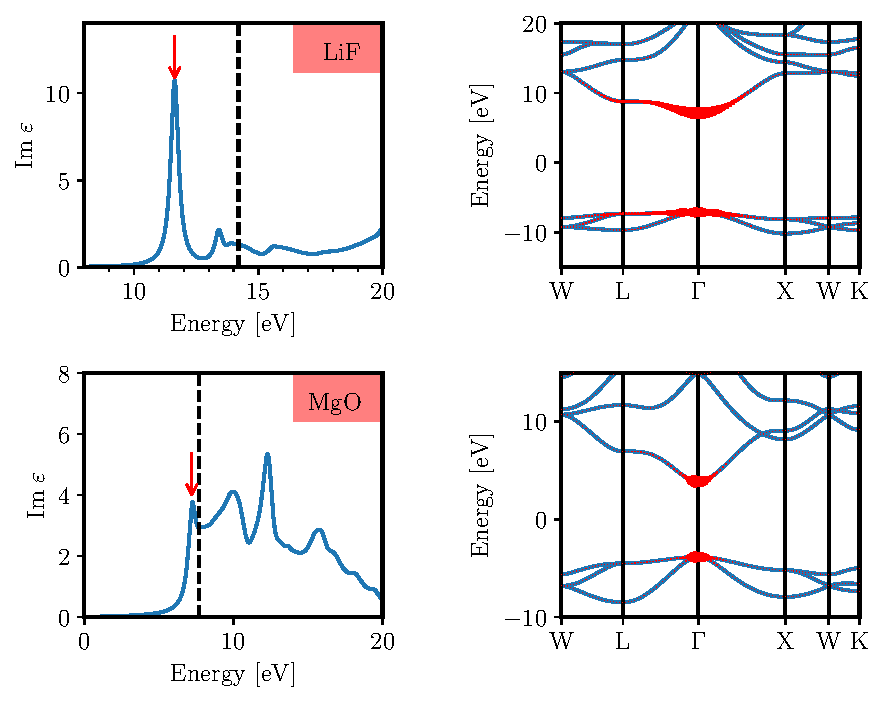
\includegraphics{work/plots/spectra/spectrum_lif_mgo.pdf}
\caption[Optical spectrum and electron-hole coupling coefficients of the first excitation in LiF and MgO.]{Left panels: Imaginary part of the dielectric function of LiF (top) and MgO (bottom).  The fundamental band gaps are marked by  dashed lines and the positions of the lowest-energy excitations by red arrows. Broadenings of 0.2\,eV (LiF) and 0.3\,eV (MgO) are applied. Right panels: Electron-hole coupling coefficients of the  lowest-energy excitation projected onto the band structure. The coupling coefficients are represented as circles, their size is proportional to the magnitude of the coefficients.\label{spectrum_figure}}
\end{figure}
Each electron-hole excitation obtained from the solution of the BSE is expressed as an expansion into independent-particle transitions (Eq.\;\eqref{eh_wf_expansion}). The expansion coefficients are given by the BSE eigenvectors $A^\lambda_{vc\k}$ corresponding to one $v\k\rightarrow c\k$ transition.  For an analysis of excitonic states, it is therefore convenient to introduce the electron-hole coupling coefficients  $w^\lambda_{v\k}$ and $w^\lambda_{c\k}$,  which define the contribution of a given valence or conduction state to the exciton, respectively. In terms of the BSE eigenvectors, they are computed as
%
\begin{equation}
    w^\lambda_{c\k} = \sum_v |A^\lambda_{vc\k}|^2, \qquad w^\lambda_{v\k} = \sum_c |A^\lambda_{vc\k}|^2.
\end{equation}
%
Exemplary, the coupling coefficients projected onto the band structure for the excitonic ground states in LiF and MgO are shown in Figure~\ref{spectrum_figure}, the results for the other materials can be found in Appendix\;\ref{app_excana}.  Additionally, the imaginary part of the dielectric function is shown, where the position of the exciton is marked. In LiF, the first exciton appears at 11.6\,eV and is, therefore, responsible for the large peak in the dielectric function shown in the upper panel. The largest coefficients can be found for transitions from the  valence band maximum (VBM) to the conduction band minimum (CBM) around $\Gamma$, but also transitions in some distance from the BZ center contribute significantly to this exciton. Due to the broad distribution of the coupling coefficients, moderately dense sampled grids (1000-2000 $\k$-points in total) suffice to describe the variation of the excitonic wave function $A^\lambda_{vc\k}$ in reciprocal space and, in turn, to converge the binding energy.\par
Turning to MgO, we find the first excitation at 7.2\,eV. Being a bright excitation, this exciton is responsible for the first peak of the spectrum, which is shown on the left-hand side of the lower panel in Figure~\ref{spectrum_figure}.  As can be seen from the figure, this exciton consists mostly of strongly localized transitions from the VBM to the CBM around $\Gamma$, and other bands contribute only to a much lower extent. Similar observations are made for the other low-binding energy materials GaN, ZnS, and ZnO. This poses a severe problem for computing converged values of the excitonic binding energy as very dense samplings around the center of the BZ are needed to obtain a converged value of the binding energy.\par
%
\begin{figure}[t]
\captionsetup{format=plain}
\centering
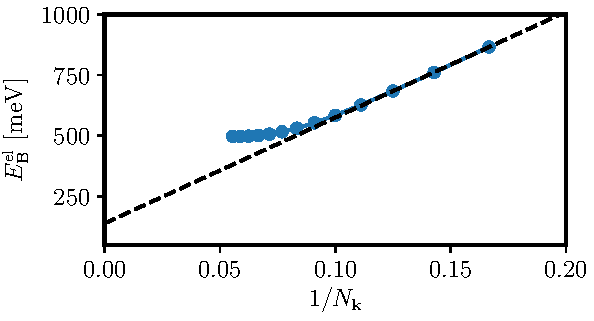
\includegraphics{work/plots/mgo_conv.pdf}
\caption[Excitonic binding energy, $E^\text{el}_\text{B}$, in MgO versus the inverse number of $\k$-points.]{Excitonic binding energy, $E^\text{el}_\text{B}$, of the first exciton in MgO computed with pure electronic screening versus the inverse number of $\k$-points, $N_\k$, in one direction. A~linear extrapolation using the five highest points is shown as dashed line. \label{conv_mgo}}
\end{figure}
%
As an example, Figure~\ref{conv_mgo} shows the excitonic binding energy $E^\text{el}_\text{B}$ in MgO, computed with pure electronic screening on a grid of $N_\k\!\times\!N_\k\!\times\!N_\k$ $\k$-points, versus 1/$N_\k$. It can be seen that the binding energy decreases linearly for coarse grids up to a sampling of 10$\times$10$\times$10 points and only for very dense grids a converging behavior can be observed. When increasing the grid from 17$\times$17$\times$17  to 18$\times$18$\times$18 points, the binding energy changes less than 0.5\%, which is seen as a sufficiently converged value. For the other materials with even lower binding energies, much denser grids would be necessary to reach convergence. However, such dense samplings  are computationally not affordable  with equally distributed $\k$-points, so that there were other methods developed like hybrid meshes. In the case of GaN, for instance, it was shown that the excitonic ground state can be converged by a dense sampling of an inner part of the BZ, which would otherwise require 2 million points distributed equally over the whole Brillouin zone\cite{draxl_gan}. Unfortunately, such a technique is not implemented in the current version of \exciting{}. Therefore, it is not possible to obtain properly converged values for the binding energies such that a different approach is needed to enable quantitative predictions within this thesis. It is presented in Section~\ref{subsec_compapproach}.\par
A further method used in the literature to overcome the difficulty of dense sampling is a simple extrapolation based on the linear decrease of the binding energy for coarse grids\cite{mgo_wrong_convergence} . However,  we assume that this method does not give the same binding energy as it would be obtained from a truly converged calculation. In MgO, the linear extrapolation, applied using the five highest points, is marked by a dashed line in~Figure~\ref{conv_mgo}. The extrapolation yields a value of around 140\,meV, which is far below the one of the converged system, which is around 500\,meV.
%




%---
\subsubsection{Phonon dispersions, Born effective charges, dielectric tensors}
%-----------------------------
\begin{figure}[t]
\captionsetup{format=plain}
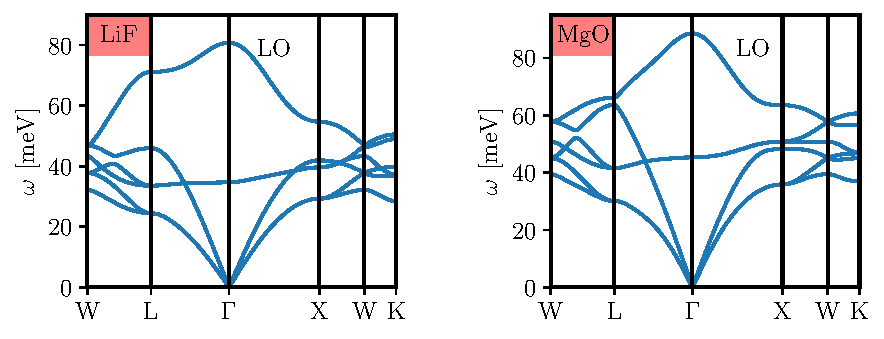
\includegraphics{work/plots/phonons/phonons.pdf}%
\caption[Phonon-dispersion curves for LiF and MgO.]{Phonon-dispersion curves for  LiF (left panel) and MgO (right panel). The longitudinal optical phonon modes most responsible for EPI are marked by~LO. \label{phonon_figure}}
\end{figure}
In Figure~\ref{phonon_figure} the phonon dispersions of LiF and MgO are shown as examples. The results for the other materials can be found in Appendix\;\ref{app_phonon}. As both crystals have a face-centered cubic structure with two atoms in the unit cell, their dispersion relations share some features. Both materials have six phonon modes, three acoustical and three optical. Two of the optical modes are transversal (TO), the other mode is longitudinal (LO), and therefore the most responsible for screening effects from phonons. At $\Gamma$, the two TO modes are degenerate and for both materials, the LO mode has a frequency of around 80\,meV.
\vfill
\newpage
Table~\ref{tab_comp_par}  shows the highest LO frequency $\omega^{\phantom{I}}_\text{LO}$ and the elements of the full static dielectric tensor $\boldsymbol{\varepsilon}_0$ and the Born effective charge tensor $\mathbf{Z}^*$. All materials exhibit large Born effective charges, which results in larger elements of the full dielectric tensors $\boldsymbol{\varepsilon}_0$ compared to the high-frequency tensor $\boldsymbol{\varepsilon}_\infty$ shown in Table~\ref{table_dynscreen}. 
 There is an overall agreement between computed and experimental values (see Table~\ref{tab_exp_data}) with only small discrepancies, in particular with regard to the Born effective charges and the phonon frequencies. A slight deviation of the computed elements of the full static dielectric tensor from the experimental counterparts can be observed, but for all materials the deviation does not exceed 10\%.  Although the dielectric tensor $\boldsymbol{\varepsilon}_0$ does not enter the construction of the screened Coulomb interaction in Eq.~\eqref{w_ph_fourier}, it is instructive to look at this quantity to quantify the effects of EPI on the excitonic binding energy: The tensor on the one hand appears in the limiting case of our first-principles approach in Eq.\;\eqref{w_ph_limit}, and on the other hand is used for evaluations within the Wannier-Mott model through Eq.\;\eqref{eb_rex}.

\begin{table}[t]
\captionsetup{format=plain}
\caption[Computed parameters relevant for EPI.]{Computed parameters relevant for EPI: Elements of the full static dielectric tensor  $\boldsymbol{\varepsilon}_0$, the Born effective charge tensor $\mathbf{Z}^*$, and the highest LO frequency. Only nonvanishing tensor elements are shown.  Parallel and perpendicular ($\parallel,\perp$) are to be understood with respect to the $\mathbf{c}$-axis of the wurtzite crystals.}
\vspace{1mm}
   \begin{tabularx}{\textwidth}{YYYY}
    \hline
    \hline
    Material  & $\boldsymbol{\varepsilon}_0$ & $\omega^{\phantom{I}}_\text{LO}$ [meV] & $|\mathbf{Z}^*|$ [a.u.] \\
    \hline
    LiF  & 9.6  & 83  & 1.1  \\
    MgO  & 10.1 & 91  & 2.0 \\
    ZnS  & 7.8  & 44  & 1.9 \\
    GaN  & 9.0 ($\perp$), 10.0 ($\parallel$)  & 91  & 2.6 ($\perp$), 2.8 ($\parallel$) \\
    ZnO  & 8.5 ($\perp$), 9.3 ($\parallel$)  & 73  & 2.1 ($\perp$), 2.2 ($\parallel$)\\
    \hline
    \hline
    \end{tabularx}
\label{tab_comp_par}
\end{table}

\vfill
\subsubsection{Computational approach for low binding energies}\label{subsec_compapproach}
%-------------------------------------
 \begin{figure}[t]
\captionsetup{format=plain}
\centering
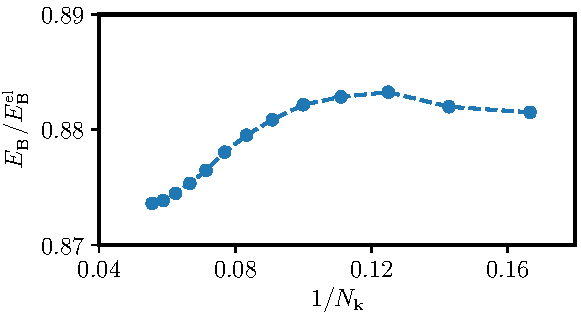
\includegraphics{work/plots/mgo_rel_conv.pdf}
\vspace{-2mm}
\caption[Ratio of the  binding energies $E_\text{B}^{\phantom{l}}$ and $E^\text{el}_\text{B}$ of the first exciton in MgO computed with and without the inclusion of EPI versus the inverse number of $\k$-points.]{Ratio of the  binding energies $E_\text{B}^{\phantom{l}}$ and $E^\text{el}_\text{B}$ of the first exciton in MgO computed with and without the inclusion of EPI  versus the inverse number of $\k$-points $N_\k$ in one direction. \label{conv_rel}}
\end{figure}
With the current implementation of \exciting{}, it is not possible to converge the low excitonic  binding energies in ZnS, GaN, and ZnO due to an insufficient $\k$-point sampling (see discussion in Section~\ref{subsec_exc_ana}). In order to make quantitative predictions within this thesis, we therefore follow an approach based on the use of  results published in the literature. More specifically, we use converged values for the binding energies $E^\text{el}_\text{B}$ and the corresponding excitation energies $E^{\lambda=0}$ obtained from the solution of the BSE using pure electronic screening. These quantities are needed as starting point for the setup of the BSE Hamiltonian in Eq.\;\eqref{h_dir_final} and for an analysis within the Wannier-Mott model in Eq.\;\eqref{eb_rex}. The key idea is that the relative effect of EPI on the binding energy is independent of the $\k$-point sampling if the same starting point is used for every grid. Therefore, also the ratio $E_\text{B}^{\phantom{l}}/E^\text{el}_\text{B}$ between the binding energy using the full screening and the binding energy with pure electronic screening is independent of the sampling. It is thus sufficient to compute both binding energies on a coarse grid and to use this ratio in order to renormalize the converged value for  $E^\text{el}_\text{B}$.\par
To justify the chosen approach, both binding energies are computed for MgO using grids of $N_\k\!\times\!N_\k\!\times\!N_\k$ points and the variation of the ratio  $E_{\text{B}}^{\phantom{l}}/E^\text{el}_{\text{B}}$ versus~$1/N_\k$ is observed. MgO is chosen, as in this material the  binding energy can be studied over a broad range of $1/N_\k$ until it converges. The corresponding values are shown in Figure~\ref{conv_rel}. For all calculations of the phonon BSE term through Eq.\;\eqref{h_dir_final}, the same starting point for the excitation energy $E^{\lambda=0}$ corresponding to a binding energy of $E^\text{el}_\text{B}=498$\,meV is used. The same number of points are used as in Figure~\ref{conv_mgo}, thus the whole range of the linear decrease up to the region where the binding energy converges is covered. As can be seen from the figure, the ratio of the two binding energies varies only very slightly with respect to the $\k$-point sampling and a change from less than 1\%-point can be observed when going from a 6$\times$6$\times$6 grid to a 18$\times$18$\times$18 grid. With increasing density of the grid, the ratio varies less, as for a large number of $\k$-points the two binding energies are converged. Also for the other materials, the ratio of the binding energies varies only very slightly with increasing number of mesh points, and the aforementioned procedure is therefore applied to these materials. The literature values for the binding energy corresponding to the used initial excitation energies can be found in Table~\ref{tab_wm_vs_full} in the next section.\par
 \begin{table}[t]
\captionsetup{format=plain}
\caption[High-frequency dielectric tensor $\boldsymbol{\varepsilon}_\infty$ computed in \exciting{} and in the literature.]{Components of the high-frequency dielectric tensor $\boldsymbol{\varepsilon}_\infty$ as computed in \exciting{} compared to experimental values. For ZnS, GaN, and ZnO, additionally literature values\cite{draxl_gan,zns_bse,zno_bse} are shown, which stem from the publications serving as reference for the binding energy $E^\text{el}_\text{B}$. Parallel and perpendicular ($\parallel,\perp$) are to be understood with respect to the $\mathbf{c}$-axis of the wurtzite crystals. For experimental references see Table~\ref{table_dynscreen}.}
\vspace{1mm}
    \centering
    \begin{tabularx}{\textwidth}{YYYY}
    \hline
    \hline
     Material & \exciting{} & Literature & Experiment \\
     \hline
    LiF & 1.8 & -   & 1.9 \\
    MgO & 2.7 & - & 2.9\\
    ZnS & 4.9 & 5.1  & 5.1 \\
    GaN & 4.8 ($\perp$), 4.9 ($\parallel$) & 5.2 ($\perp$),  5.3 ($\parallel$) & 5.4 ($\perp$), 5.8 ($\parallel$)\\
    ZnO & 3.7 ($\perp$), 3.7 ($\parallel$) & not published  &  3.7 ($\perp$), 3.8 ($\parallel$)\\
    \hline
    \hline
    \end{tabularx}
    \label{tab_highfreq_screen}
\end{table}
It is clear that this procedure does not provide a fully quantitative way to evaluate the effects of EPI since results of different codes using different computational parameters are used. Nevertheless, the BSE implementation within \exciting{} has been shown to be in good agreement with previous works at the same level of theory\cite{Vorwerk_2019} and therefore the findings are seen to be not just of a qualitative nature.\par
This assumption is supported by the values of the high-frequency dielectric tensors  $\boldsymbol{\varepsilon}_\infty$, which agree among the different computations. The components of the dielectric tensors of all investigated materials and their experimental counterparts are shown in Table~\ref{tab_highfreq_screen}. One can observe a slight underestimation of the high-frequency dielectric tensor as computed in \exciting{} compared to the reference values from literature calculations and experiment.  The underestimation  can be attributed to the use of quasiparticle corrections of the electronic structure. Evaluating the screening using the Kohn-Sham band structure, however, a much stronger overestimation is found. Overall, the values are close enough to expect that the published binding energies deviate only slightly from those which would have been obtained with \exciting{} using a dense sampling.
\vfill
%

%-------------------------
%-----------------------------------

%-----------------------------
\subsubsection{Renormalization of the binding energy}
%-------------------------

In Table~\ref{tab_wm_vs_full}, excitonic binding energies  computed with pure electronic screening $E_\text{B}^\text{el}$ and with the additional contribution from EPI $E_\text{B}^{\phantom{l}}$ are presented. The values obtained from our full first-principles approach (BSE) are compared with values obtained from the Wannier-Mott (WM) model and experimental values. The initial excitation energies for the setup of the BSE Hamiltonian (Eq.\;\eqref{h_dir_final}) and the computation within the WM model (Eq.\;\eqref{eb_rex})  are obtained from a BSE calculation employing pure electronic screening. For ZnS, GaN, and ZnO, these values correspond to binding energies  $E^\text{el}_\text{B}$ extracted from the literature\cite{draxl_gan,zns_bse,zno_bse}. The presented values for $E_\text{B}^{\phantom{l}}$ are obtained from one-shot calculations for both the BSE and WM approach, \textit{i.e.}, the binding energies are not updated. The convergence with respect to an update of the binding energy is discussed in Section~\ref{subsec_selfconsistent}.\par
\begin{table}[t]
\captionsetup{format=plain}
 \caption[Binding energies $E_\text{B}^{\phantom{l}}$ as obtained from first-principles calculations, the Wannier-Mott model and experiment.]{Binding energies in meV: $E^\text{el}_\text{B}$ computed with pure electronic screening, and $E_\text{B}^{\phantom{l}}$  with the additional effects of EPI. Results are obtained from our first-principles calculations (BSE) and the Wannier-Mott (WM) model. Experimental (Expt.) values are shown for comparison. Starting values $E^\text{el}_\text{B}$ are extracted from the literature for ZnS\cite{zns_bse}, GaN\cite{draxl_gan}, and ZnO\cite{zno_bse}. For experimental references see Table~\ref{table_dynscreen}. \label{tab_wm_vs_full}}
\vspace{1mm} 
 \centering
 \begin{tabularx}{\textwidth}{YYYYY}
    \hline
    \hline
%  \multicolumn{1}{c}{}& \multicolumn{2}{c}{BSE} & \multicolumn{1}{c}{WM } & \multicolumn{1}{c}{Expt.}\\
%  \hline
 Material & $E^\text{el}_\text{B}$ (BSE) & $E_\text{B}^{\phantom{l}}$ (BSE)  & $E_\text{B}^{\phantom{l}}$ (WM)  &  $E_\text{B}^{\phantom{l}}$ (Expt.) \\
\hline
LiF & 2568   & 2495 &  2502  & 1600\\
MgO & 498    & 435  &  439   & $\,\;85$\,-\,$100$\\
ZnS & 52     & 43   &  42    & $32$\,-\,$36$\\
GaN & 37     & 24   &  21    & $18$\,-\,$28$\\
ZnO & 68     & 48   &  45    & $50$\,-\,$60$\\
    \hline
    \hline
\end{tabularx}  
\end{table}
%
From the values in Table~\ref{tab_wm_vs_full}, we see that the exciton binding energy decreases in all of the investigated materials when EPI is included. However, large differences become apparent with regard to the  magnitude of effects. While a reduction of the binding energy  of around 30\% can be found in GaN and ZnO, there is only a decrease of less than 20\% in MgO and ZnS. In LiF, the binding energy decreases only about~3\%. For these differences, the different lattice polarizabilities, and, in particular,  the dynamics of the screening are responsible. These effects are further discussed in Section~\ref{subsec_dyn_pol_effects}. It can be found that the results obtained from our first-principles approach are close to those obtained within the WM model. For LiF, MgO, and ZnS, only small (relative) deviations can be observed, whereas larger ones are found for GaN and ZnO. As in the two latter materials the effects of EPI are stronger, the deviations between the two approaches become more pronounced. Overall, however, there is a good agreement between the results. When comparing these values, one should be aware of the fact that the ground-state excitons in the investigated materials (except LiF) fulfil the main assumption of the WM model, \textit{i.e.}, they are mostly composed of transitions from the valence band maximum to the conduction band minimum (see Section~\ref{subsec_exc_ana}). Furthermore, only a small number of LO phonon modes is present. Therefore, the assumptions made in Section~\ref{subsec_wm} to solve the WM model  analytically hold such that comparable values can be found as from a  full BSE solution. Our results are further supported by a recently published study\footnote[2]{This study also served as a reference for the converged value of the binding energy $E^\text{el}_\text{B}$ with pure electronic screening.} of the effects of EPI on the excitonic binding energy in ZnS, where a comparable result of 42\,meV was found\cite{zns_bse}.\par 

Moreover, it can be observed that the computed binding energies in ZnS, GaN, and ZnO come much closer to the experimental range when EPI is included, which demonstrates the importance of correctly capturing these effects. In the case of GaN, it should be noted that the literature value of $E^\text{el}_\text{B}=37$\,meV was obtained using a dielectric tensor whose elements are about 10\% smaller than the experimental values (see Table~\ref{tab_highfreq_screen}). An approximate reduction of the binding energy by 8\,meV  ($E^\text{el}_\text{B}=29$\,meV) is reported in the publication when using the experimental values for the high-frequency dielectric tensor\cite{draxl_gan}. Using this value as a starting point, a binding energy of $E_\text{B}^{\phantom{l}}=19$\,meV is obtained. 


For MgO and LiF, the discrepancies between computed and experimental values are still large. However, we do not attribute this observation to an erroneous treatment of EPI but to an overestimation of the binding energy computed with pure electronic screening. Using \exciting{}, binding energies $E^\text{el}_\text{B}$  of 498\,meV (MgO) and 2.568\,eV (LiF) are obtained. Similar large values of 430\,meV and 2.050\,eV are reported in the literature\cite{fuchs_08,low_cost}, where the deviation from our results can be mainly traced back to the fact that we used slightly lower dielectric constants (2.7 compared to~3.0  for MgO and 1.8  compared to around~2.0 for LiF). Within the hydrogen-like WM model, where $E^\text{el}_\text{B}\propto\varepsilon^{-2}_\infty$ (see Eq.\;\eqref{wm_rex}), the effect of larger dielectric constants can be estimated, reducing our values to binding energies of~410\,meV  (MgO) and~2100\,meV (LiF), respectively.  As in the literature\cite{fuchs_08,low_cost} the used values for $\varepsilon_\infty$ are even larger than the experimental ones (1.9 for LiF and 2.9 for MgO), we assume that the binding energies $E^\text{el}_\text{B}$ are overestimating the true values  $E_\text{B}^{\phantom{l}}$ not only by neglecting long-range EPI but also by other effects. It is, however, difficult to specify where this overestimation stems from. One possible reason could be the neglection of the short-range contribution to the electron-phonon coupling in this work. From an evaluation of Eq.\;\eqref{eb_rex}, it can be found that values of around $E^\text{el}_\text{B}=140$\,meV (MgO) and $E^\text{el}_\text{B}=1.7$\,eV (LiF) would correspond to a full binding energy $E_\text{B}^{\phantom{l}}$ within the range of experimental values.\par

\subsubsection{Effects of screening dynamics and lattice polarizability}\label{subsec_dyn_pol_effects}
In the interest of analyzing the effects of  lattice polarizability and dynamical screening  on the excitonic binding energy, we again compare the binding energy computed with pure electronic screening  $E_\text{B}^\text{el}$ with the full binding energy $E_\text{B}^{\phantom{l}}$ including effects from~EPI. As our approach accounts for Fr\"ohlich coupling, one expects that the polarizability of the lattice, \textit{i.e.}, the contribution of the lattice to the dielectric tensor, should determine how strong EPI affects the binding energy. In the derivation of the phonon contribution to the BSE Hamiltonian in Section~\ref{dir_int_ph}, it was further found that the impact of EPI on the binding energy depends on the ability of the lattice to follow the exciton formation. In order to illustrate the dynamical effects, we make use of the WM model. From Eq.\;\eqref{eps_eff}, we recall that in this model the effective dielectric constant screening the exciton formation can be defined by~$E_\text{B}^{\phantom{l}} = E^\text{el}_\text{B}\cdot(\varepsilon_\infty/\varepsilon_\text{eff})^2$. Based on this relation, we introduce the parameter~$f_\text{lat}$~as
%
\begin{equation}\label{flat}
    \varepsilon_\text{eff} = \varepsilon_\infty +f_\text{lat}\cdot(\varepsilon_0 - \varepsilon_\infty), 
\end{equation}
%
which takes values between 0 and 1, and can be interpreted as the fraction of the lattice polarizability contributing to the screening. While a value of 0 indicates that only electrons screen the exciton formation ($\varepsilon_\text{eff}=\varepsilon_\infty$), a value of 1 occurs if the whole lattice polarizability contributes to the screening($\varepsilon_\text{eff}=\varepsilon_0$). All values between 0 and 1 correspond to a fractional contribution of the lattice polarizability. 

\begin{table}[t]
\captionsetup{format=plain}
 \caption[Physical quantities determining the impact of EPI on the excitonic binding energy renormalization.]{Ratio between binding energies $E_\text{B}^{\phantom{l}}/E_\text{B}^\text{el}$ and physical quantities determining the impact of EPI on the binding energy.\label{tab_strength}}
 \vspace{1mm}
 \centering
 \begin{tabularx}{\textwidth}{YYYYY}
    \hline
    \hline
 Material  & $\omega^{\phantom{I}}_\text{LO}/E^\text{el}_\text{B}$& $f_\text{lat}$ [\%] & $\varepsilon_0/\varepsilon_\infty$ & $E_\text{B}^{\phantom{l}}/E_\text{B}^\text{el}$ \\
\hline
LiF    & 0.03 & 0.3 &  5.4   & 0.97 \\
MgO    & 0.2  & 2 &  3.8   & 0.87   \\
ZnS    & 0.8  & 17 &  1.6   & 0.83  \\
GaN    & 2.5  &  25  & 1.9   & 0.65  \\
ZnO    & 1.1  &  14 & 2.4   & 0.70  \\
    \hline
    \hline
\end{tabularx}  
\end{table}
%
In Table~\ref{tab_strength},  the ratios between the highest LO frequency and the binding energy $\omega^{\phantom{I}}_\text{LO}/E_\text{B}^{\text{el}}$,  between the averaged full static dielectric constant and the high-frequency constant $\varepsilon_0/\varepsilon_\infty$, and  between the full binding energy including effects from EPI and the binding energy computed with pure electronic screening $E_\text{B}^{\phantom{l}}/E_\text{B}^\text{el}$ as obtained from BSE are  presented. Additionally, the parameter $f_\text{lat}$ is shown. It can be observed that the larger  $\omega^{\phantom{I}}_\text{LO}$ is compared to  $E_\text{B}^{\text{el}}$, the higher is the lattice contribution $f_\text{lat}$ and, in turn, the smaller is $E_\text{B}^{\phantom{l}}$ compared to $E^\text{el}_\text{B}$. This can be interpreted as follows:~For large binding energies, the exciton formation is so fast that the lattice is unable to form a polarization cloud around the electron-hole pair. The contribution of the lattice polarizability to the screening is very small and the screening stems only from electrons. For small binding energies, in contrast, the exciton formation is slow such that the lattice vibrations have enough time to follow the motion of electron and hole. Consequently, the screening significantly increases when EPI is considered. In LiF, the phonon frequency is much smaller than the binding energy such that  the lattice can follow the fast exciton formation to a very low extent. The binding energy reduces by solely~3\% under the inclusion of EPI as only 0.3\% of the lattice polarizability contribute to the screening.  In the other materials, a larger fraction of the lattice polarizability is able to follow the exciton formation as phonon frequencies and binding energies are closer. In GaN, the phonon frequency is more than 2 times larger than the binding energy, which results in a reduction of the binding energy of 35\%. The  lattice is partly able to follow the slow exciton formation, 25\% of the lattice polarizability contribute to the screening.\par 

Moreover, it can be seen that the reduction from $E^\text{el}_\text{B}$ to  $E_\text{B}^{\phantom{l}}$ indeed depends on the lattice polarizability and, hence, the ratio of the dielectric constants $\varepsilon_0/\varepsilon_\infty$. The larger~$\varepsilon_0$ is compared to $\varepsilon_\infty$, the stronger is the influence of EPI resulting in a larger reduction of the binding energy. Looking at ZnS and ZnO, having comparable ratios $\omega^{\phantom{I}}_\text{LO}/E^\text{el}_\text{B}$ of 0.8 and 1.1 but different ratios $\varepsilon_0/\varepsilon_\infty$ of 1.6 and 2.4, respectively, we see that in ZnO  the binding energy is reduced by 30\%, whereas in ZnS only a reduction of 17\% can be observed. A comparable value is found for MgO due to the large lattice polarizability ($\varepsilon_0/\varepsilon_\infty=3.8$), although in this material the binding energy is 5 times larger than the LO phonon frequency. In LiF, the large lattice polarizability leads to a reduction of the binding energy of 3\%, despite the fact that the phonon frequency is almost negligible compared to the huge binding energy.\par

To demonstrate the importance of correctly treating the screening due to EPI, Table~\ref{tab_eb_dynscreen} shows the binding energy of the various materials computed without and with the inclusion of dynamical effects (the latter are equal to the values shown in Table~\ref{tab_wm_vs_full}). The case of neglecting dynamical effects corresponds to setting the weight in the second and third line of the phonon contribution to the direct BSE term Eq.\;\eqref{h_dir_final} equal to one.
%
\begin{table}[t]
\captionsetup{format=plain}
 \caption[Binding energies computed with and without treatment of  dynamical screening effects.]{Binding energies $E_\text{B}^{\phantom{l}}$ in meV computed with  dynamical (dyn.) and static (stat.) treatment of  screening effects. For comparison, the values calculated with pure electronic screening $E_\text{B}^\text{el}$ and the experimental (Expt.) values are shown as~well. \label{tab_eb_dynscreen}}
 \vspace{1mm}
 \centering
 \begin{tabularx}{\textwidth}{YYYYY}
    \hline
    \hline
 Material  & $E_\text{B}^\text{el}$ &   $E_\text{B}^{\phantom{l}}$ (dyn.) &  $E_\text{B}^{\phantom{l}}$ (stat.) &  $E_\text{B}^{\phantom{l}}$ (Expt.) \\
\hline
LiF & 2568  & 2495  & 1520 & 1600\\
MgO & 498   & 435   & 92  & $\,\;85$\;-\;$100$\\
ZnS & 52    & 43    & 31  & $34$\,-\,$37$\\
GaN & 37    & 24    & 18  & $18$\,-\,$28$\\
ZnO & 68    & 48    & 26  & $50$\,-\,$60$\\ 
    \hline
    \hline
\end{tabularx}  
\end{table}
%
It becomes evident that dynamical effects have a strong influence on the renormalization of the excitonic binding energy. In particular for LiF and MgO, materials with large (computed) binding energies, the neglection of the dynamics leads to binding energies much smaller than the values computed with dynamical screening. This can be explained by the fact that without dynamical effects each mode fully contributes to the screening, whereas in the dynamical case the lattice vibrations follow the exciton formation only to a very low extent in these materials. For LiF and MgO, it can further be observed that the binding energies computed under the assumption of static screening are very close to the experimental values. However, this is only the case due to a strong overestimation of the binding energy $E_\text{B}^\text{el}$ computed with pure electronic screening, as already discussed in the preceding section. For ZnS, GaN, and ZnO, the neglection of dynamical effects similarly leads to a stronger renormalization of the binding energies. At variance with LiF and MgO,  the additional screening effects are smaller, as also in the dynamical case the lattice follows the exciton formation to a large extent as phonon frequencies and binding energies are in the same order of magnitude.\par
Nevertheless, neglecting dynamical effects leads to an underestimation of the binding energies in ZnO and ZnS. In GaN, the computed value moves to the lower limit of the experimental range when a starting value of  $E_\text{B}^\text{el}=37$\,meV is used. However, this value is likely to be overestimated due to an underestimation of the dielectric tensor in the RPA screening (see the discussion in the previous section). Assuming that the correct value is around $E_\text{B}^\text{el}=28$\,meV, a binding energy of $E_\text{B}^{\phantom{l}}=14$\,meV is obtained when dynamical effects of the phonon screening are neglected. Similar to the case of ZnS and ZnO, this value also is below the experimental values, which were found in the range of 18\,-\,28\,meV.\par
In conclusion, the results discussed in this section show that a correct treatment of dynamical effects in the phonon part of the screening is crucial in order not to overestimate the renormalization of the excitonic binding energy due to EPI. It should be stressed  that this is true for materials with large and small binding energies alike, although, for LiF and MgO, the neglection of dynamical effects yields results much closer to experiment which indicates that additional effects might be present. 

\subsubsection{Self-consistent solution of the BSE}\label{subsec_selfconsistent}
%
\begin{figure}[t]
\captionsetup{format=plain}
\centering
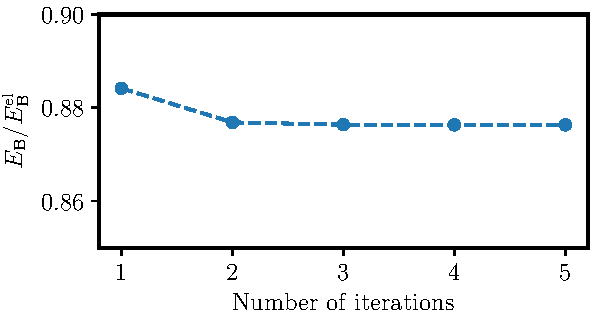
\includegraphics{work/plots/mgo_iteration.pdf}
\caption{Ratio of the binding energies $E_\text{B}^{\phantom{l}}/E^\text{el}_\text{B}$  of the first exciton in MgO versus the number of iterations.\label{iteration_conv}}
\end{figure}
%
As already discussed in Section~\ref{implement_subsec}, the BSE has, in principle, to be solved self-consistently, as the direct term itself depends on the BSE solutions $E^\lambda$.  In Figure~\ref{iteration_conv}, the ratio $E_\text{B}^{\phantom{l}}$ to the initial of value $E^\text{el}_\text{B} = 498$\,meV for the first exciton in MgO is shown versus the number of iterations. The first input energy for the ground-state excitation is the one obtained from pure electronic screening and corresponds to $E^\text{el}_\text{B}$. The resulting binding energy $E_\text{B}^{\phantom{l}}$ after the inclusion of EPI serves as the input energy of the next calculation. From the figure, we can see that sufficient convergence is reached after a few iterations. The reduction between the first to the fourth iteration is roughly 1\% with a change below 0.02\,meV from the third to the fourth iteration. A similar convergence behavior is observed for the other materials. Only one iteration is therefore seen to be satisfactory, as for ZnS, GaN, and ZnO exact numbers are in any case out of reach due to insufficient $\k$-point sampling. Moreover, even for fully converged calculations the error of excitonic binding energies from the solution of the BSE is presumably larger than the changes shown in Figure~\ref{iteration_conv} being  below~1\%.  

\vspace{\fill}
%-------------------------

\newpage
\phantom.
\vspace{3cm}
%----------------------------------
\section{Conclusions and outlook}
%----------------------------------
In the present thesis, a first-principles approach was developed accounting for the influence of electron-phonon interactions (EPI) on excitonic binding energies in polar materials. The derivation includes the coupling to all modes, and no assumptions about the crystal symmetry were made. This represents important progress as previous models are usually based on the coupling to specific modes in isotropic systems. A central element was the derivation of a frequency-dependent phonon contribution to the screened Coulomb interaction, which is completely general and does not require any assumptions about the material. Starting from the Fan-Migdal self-energy of electron-phonon coupling, defining screening effects stemming from phonons on a fundamental level, a real-space expression for the screened Coulomb interaction could be extracted. A leading idea was the expansion in terms of the electron-phonon matrix element, which allows the connection of the developed formalism to the standard notation. The corresponding contribution of phonons to the direct BSE term was derived, which results in an energy-dependent term due to the inclusion of frequency dependence. Being valid for all types of materials, we applied the developed formalism to polar crystals. Here, an explicit expression for the long-range electron-phonon matrix element exists, which is a generalized version of the Fr\"ohlich coupling.  It could be shown that a widely-used screening model is contained as a limiting case in our approach.  The derived expressions for the phonon contribution to screened Coulomb interaction and the direct BSE term were implemented into the all-electron code \exciting{}. \par
With the  developed approach, effects of EPI on the excitonic binding energy of LiF and the prototypical polar semiconductors MgO, GaN, ZnS, and ZnO were investigated. Except LiF, the ground state excitons in these materials have relatively low binding energies in the order of 100\,meV and are rather delocalized in real space. Hence, the excitons are composed of transitions  strongly localized around the center of the Brillouin zone, which requires an extremely dense sampling of this region  in order to converge the binding energy. In the current implementation of \exciting{}, such a sampling technique  is not implemented and converged computations of binding energies are therefore prohibitive for ZnS, GaN, and ZnO. Nevertheless, a computational approach based on the use of converged values published in the literature allowed quantitative predictions also for these materials. Specifically, converged values for the binding energies computed with pure electronic screening were used, and their ratio to the values obtained when including EPI could be computed. Both binding energies computed with \exciting{} and those extracted from the literature overestimate the binding energy if effects from EPI are neglected. After the inclusion of EPI, the computed values come significantly closer to or reach exactly the experimental range for the three materials ZnS, GaN, and ZnO. For LiF and MgO, however, the reduction of the binding energy is not large enough to reach the experimental range. Here, it is assumed that other physical effects, which we do not account for, have an influence on the binding energy as well. However, it is very difficult to specify wh ere the overestimation stems from. One possible reason could be the neglection of the short-range contribution to the electron-phonon coupling in this work. \par 
An analysis within the simplifying Wannier-Mott model yields values very close to those obtained from the first-principles approach. Furthermore, it could be shown that the developed method correctly accounts for dynamical screening effects: In LiF, where the binding energy is above of 2\,eV, EPI reduces the binding energy by less than 1\% as the lattice is unable to follow the fast exciton formation. In the other materials, reductions up to 30\% could be observed. Using results from different codes, the findings are not fully quantitative. However, since the different BSE codes have been shown to produce similar results for other calculations, the deviations are expected to be small.\par
Due to the aforementioned computational difficulties, the effects of EPI on excitonic binding energies were analyzed only for small polar binary compounds, which are already well studied in the literature. We intend to extend the study to more complex polar materials such as $\text{Ga}_2\text{O}_3$ and perovskites, where strong effects of EPI on excitons can be expected.  The implementation of more flexible grids in reciprocal space is urgently needed in this context.  A future goal is also the inclusion of screening effects on the whole optical spectrum, as in the current approach one is limited to study effects on a specific excitation. Furthermore, as temperature effects on excitonic binding energies can be observed in experiments\cite{exciton_perovskites}, it would be interesting to advance the developed formalism in this regard.
%-------------------------
%-------------------------